\documentclass{article}
\usepackage{graphicx}
\usepackage{amsmath,amsthm,amssymb}
\usepackage[font=small,labelfont=bf]{caption}
\usepackage{tikz}
\usetikzlibrary{calc, angles, quotes, shapes.geometric}
\usepackage{tkz-euclide}
\usepackage{float}
\usepackage[margin=1in]{geometry}
\usepackage{gensymb}
\usepackage{fancyhdr}
\pagestyle{fancy}
\fancyhead[R]{Enoch Yu}
\pagenumbering{gobble}
\usepackage{enumitem}
\newtheorem{theorem}{Theorem}[section]
\newtheorem{lemma}[theorem]{Lemma}
\newtheorem{sublemma}{Lemma}[section]
\newtheorem{proposition}{Proposition}
\newtheorem{corollary}{Corollary}[theorem]
\newenvironment{solution}{\begin{trivlist}\item[]{\bf Solution}}{\qed \end{trivlist}}
\newcommand{\verteq}{\rotatebox{90}{$\;\;=\;\;$}}
\newcommand*\circled[1]{\tikz[baseline=(char.base)]{
            \node[shape=circle,draw,inner sep=1pt] (char) {#1};}}
\newcommand{\triangled}[1]{\tikz[baseline=(char.base)]{
            \node[shape=regular polygon, regular polygon sides=3, draw, inner sep=0.2pt] (char) {#1};}}

\title{Problem Set 5}
\author{Enoch Yu}
\date{May 2025}

\begin{document}

\section*{Problem}
In $\triangle{ABC}$, $D$ is the mid-point of $BC$ and $m$ is a point of $AD$. The extension of $BM$ meets $AC$ at $N$, and $AB$ is tangent to the circumcircle of $\triangle{BCN}$. If $BC=8$ and $BN=6$, find the length of $BM$.
\begin{solution}
\begin{center}
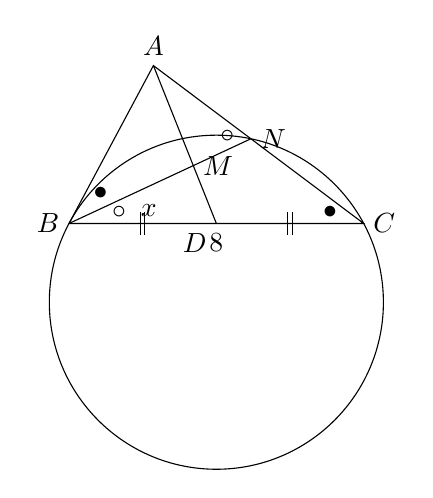
\begin{tikzpicture}
    \coordinate (A) at (-0.79959, 2.00512);
    \coordinate (B) at (-1.87083, 0);
    \coordinate (C) at (1.87083, 0);
    \coordinate (D) at (0,0);
    \coordinate (N) at (0.43847, 1.07551);
    \coordinate (M) at (-0.29303, 0.73483);

    \draw (0,-1) circle (2.12132034356);

    \draw (A) -- (B) -- (C) -- cycle;
    \draw (A) -- (D);
    \draw (B) -- (N);

    \node[above] at (A) {$A$};
    \node[left] at (B) {$B$};
    \node[right] at (C) {$C$};
    \node[below left] at (D) {$D$};
    \node[right] at (N) {$N$};
    \node[right] at (M) {$M$};

    \node[below] at ($(B)!0.5!(C)$) {8};
    \node[below right] at ($(B)!0.5!(M)$) {$x$};

    \tkzMarkSegment[pos=.5, mark=||](B, D);
    \tkzMarkSegment[pos=.5, mark=||](D, C);

    \draw pic["$\circ$", angle eccentricity=0.6] {angle=A--N--B};
    \draw pic["$\circ$", angle eccentricity=1.3] {angle=C--B--N};
    \draw pic["$\bullet$", angle eccentricity=1.1] {angle=N--B--A};
    \draw pic["$\bullet$", angle eccentricity=0.9] {angle=N--C--B};
\end{tikzpicture}
\end{center}
\textbf{Key Word} Mass Point, Menelaus's Theorem, Similar Triangle
\\
\begin{tikzpicture}[scale=1.4]
    \coordinate (A) at (-0.3, 0.95);
    \coordinate (B) at (-0.5, -0.866);
    \coordinate (C) at (0.85, -0.54);
    \coordinate (D) at (2.15, 1.5);
    \coordinate (E) at (0.25,-1.5);
    \coordinate (O) at (0,0);
    
    \draw[fill=none] (0,0) circle (1.0);
    
    \draw (A) -- (B) -- (C) -- cycle;
    \draw (D) -- (E);
    
    \draw pic[draw=black, radius=0.1cm, "$\alpha$", angle eccentricity=1.4] {angle=B--A--C};
    \draw pic[draw=black, radius=0.1cm, "$\alpha$", angle eccentricity=1.4] {angle=B--C--E};
    \draw pic[draw=black, radius=0.1cm, "$\beta$", angle eccentricity=1.4] {angle=C--B--A};
    \draw pic[draw=black, radius=0.1cm, "$\beta$", angle eccentricity=1.4] {angle=D--C--A};
    
    \node[anchor=north west] at (-2.2, 2.7) {\textbf{Property I}};
    
    \coordinate (SW) at (current bounding box.south west);
    \coordinate (NE) at (current bounding box.north east);
    \path[draw=black] 
    ($(SW)+(-0.5,-0.5)$) rectangle ($(NE)+(0.5,0.53)$);
\end{tikzpicture}
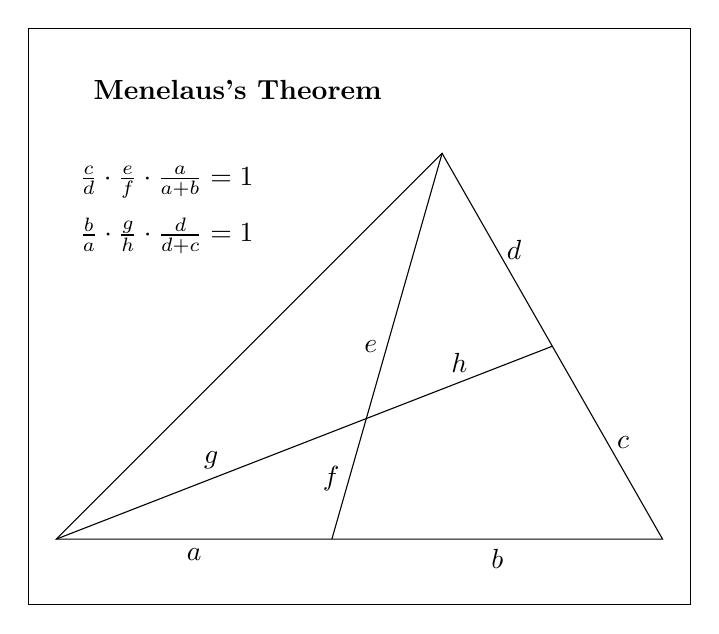
\begin{tikzpicture}[scale=0.7]
    \coordinate (A) at (1,7);
    \coordinate (B) at (-6,0);
    \coordinate (C) at (5,0);
    \coordinate (D) at (-1,0);
    \coordinate (E) at (3, 3.5);
    \coordinate (F) at (-0.375, 2.1875);

    \draw (A) -- (B) -- (C) -- cycle;
    \draw (A) -- (D);
    \draw (B) -- (E);

    \node[left] at ($(A)!0.5!(D)$) {$e$};
    \node[left] at ($(F)!0.5!(D)$) {$f$};
    \node[above] at ($(B)!0.5!(F)$) {$g$};
    \node[above] at ($(F)!0.5!(E)$) {$h$};
    \node[below] at ($(B)!0.5!(D)$) {$a$};
    \node[below] at ($(D)!0.5!(C)$) {$b$};
    \node[right] at ($(C)!0.5!(E)$) {$c$};
    \node[right] at ($(E)!0.5!(A)$) {$d$};

    \node[anchor=north west] at (-5.5, 8.5) {\textbf{Menelaus's Theorem}};
    \node[anchor=south] at (-4, 6) {$\frac{c}{d}\cdot\frac{e}{f}\cdot\frac{a}{a+b}=1$};
    \node[anchor=south] at (-4, 5) {$\frac{b}{a}\cdot\frac{g}{h}\cdot\frac{d}{d+c}=1$};
    
    \coordinate (SW) at (current bounding box.south west);
    \coordinate (NE) at (current bounding box.north east);
    \path[draw=black] 
    ($(SW)+(-0.5,-0.5)$) rectangle ($(NE)+(0.5,0.78)$);
\end{tikzpicture}
\\\\
\noindent
\textbf{Solution I: Mass Point} \\
Using Property I or Power of a Point Theorem, it is evident that $AN:NC:AB=3:\frac{7}{3}:4$. Therefore, masses for each points could be assigned.
\begin{center}
    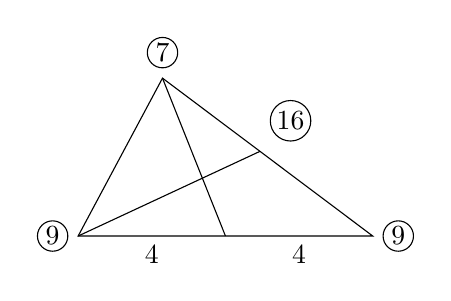
\begin{tikzpicture}
        \coordinate (A) at (-0.79959, 2.00512);
        \coordinate (B) at (-1.87083, 0);
        \coordinate (C) at (1.87083, 0);
        \coordinate (D) at (0,0);
        \coordinate (N) at (0.43847, 1.07551);
        \coordinate (M) at (-0.29303, 0.73483);

        \draw (A) -- (B) -- (C) -- cycle;
        \draw (A) -- (D);
        \draw (B) -- (N);

        \node[above] at (A) {\circled{7}};
        \node[left] at (B) {\circled{9}};
        \node[right] at (C) {\circled{9}};
        \node[above right] at (N) {\circled{16}};

        \node[below] at ($(B)!0.5!(D)$) {4};
        \node[below] at ($(D)!0.5!(C)$) {4};
    \end{tikzpicture}
\end{center}
\[
6\cdot\frac{16}{16+9}=\boxed{\frac{96}{25}}
\]
\noindent
\textbf{Solution II: Menelaus's Theorem} \\
Menelaus's Theorem may be utilized to solve the problem.
\[
\frac{4}{4}\cdot\frac{x}{6-x}\cdot\frac{9}{16}=1
\]
Therefore, $x$ could be calculated.
\begin{align*}
    \frac{4}{4}\cdot\frac{x}{6-x}\cdot\frac{9}{16}&=1 \\
    9x&=16(6-x) \\
    x&=\boxed{\frac{96}{25}}
\end{align*}
\\\\
\noindent
\textbf{Solution III: Similar Triangle} \\
A parallel line could be drawn to $AC$ from $D$.
\begin{center}
    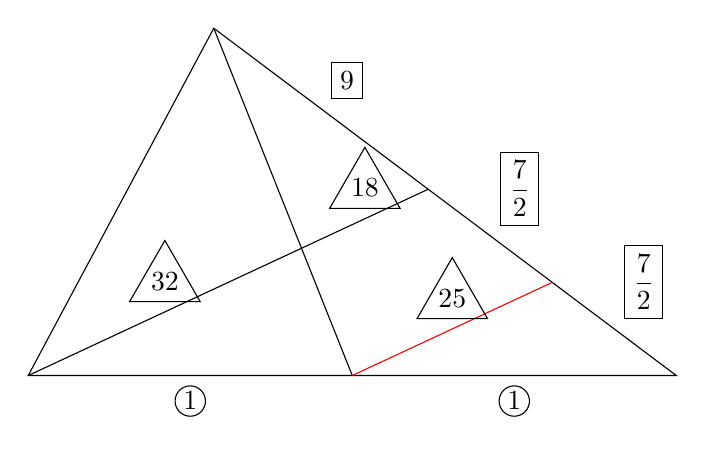
\begin{tikzpicture} [scale=2.2]
        \coordinate (A) at (-0.79959, 2.00512);
        \coordinate (B) at (-1.87083, 0);
        \coordinate (C) at (1.87083, 0);
        \coordinate (D) at (0,0);
        \coordinate (N) at (0.43847, 1.07551);
        \coordinate (E) at (1.15465, 0.53775);
        \coordinate (M) at (-0.29303, 0.73483);

        \draw (A) -- (B) -- (C) -- cycle;
        \draw (A) -- (D);
        \draw (B) -- (N);
        \draw[color=red] (D) -- (E);

        \node[below] at ($(B)!0.5!(D)$) {\circled{1}};
        \node[below] at ($(D)!0.5!(C)$) {\circled{1}};
        \node[above right] at ($(A)!0.5!(N)$) {$\boxed{9}$};
        \node[above right] at ($(N)!0.5!(E)$) {$\boxed{\frac{7}{2}}$};
        \node[above right] at ($(E)!0.5!(C)$) {$\boxed{\frac{7}{2}}$};
        \node[above] at ($(D)!0.5!(E)$) {\triangled{25}};
        \node[above] at ($(M)!0.5!(N)$) {\triangled{18}};
        \node[above] at ($(B)!0.5!(M)$) {\triangled{32}};
    \end{tikzpicture}
\end{center}
\[
BM=6\cdot\frac{32}{32+18}=\boxed{\frac{96}{25}}
\]
\end{solution}

\section*{Problem}
If $a^3-3ab^2=11$ and $b^3-3a^2b=13$, find the value of $a^2+b^2$.
\begin{solution}
\\\\
\textbf{Key Word} $\boxed{\text{DO NOT BE AFRAID TO INCREASE DEGREE}}$
\\\\
I am looking for $a^2+b^2$. However, in the given equations $a^3-3ab^2=11$ and $b^3-3a^2b=13$, There are powers with odd numbers. What should I do? I think I want to square them to make the exponents even.
\begin{align*}
    (a^3-3ab^2)^2&=a^6-6a^4b^2+9a^2b^4=121 \\
    (b^3-3a^2b)^2&=b^6-6a^2b^4+9a^4b^2=169
\end{align*}
An impulse to add the equations are created due to like terms.
\[
a^6-6a^4b^2+9a^2b^4+b^6-6a^2b^4+9a^4b^2=a^6+3a^4b^2+3a^2b^4+b^6=(a^2+b^2)^3=290
\]
Therefore, $a^2+b^2=\boxed{\sqrt[3]{290}}$
\end{solution}

\newpage
\section*{Problem}
In $\triangle{ABC}$, $P$ and $Q$ are points of $AB$ and $AC$ respectively such that $AP:PB=8:1$ and $AQ:QC=15:1$. $X$ and $Y$ are points on $BC$ such that the circumcircle of $\triangle{APX}$ is tangent to both $BC$ and $CA$, while the circumcircle of $\triangle{AQY}$ is tangent to both $AB$ and $BC$. Find $\cos{\angle{BAC}}$.
\begin{solution}
\\\\
\textbf{Key Word} Law of Cosines, Power of a Point Theorem
\begin{center}
    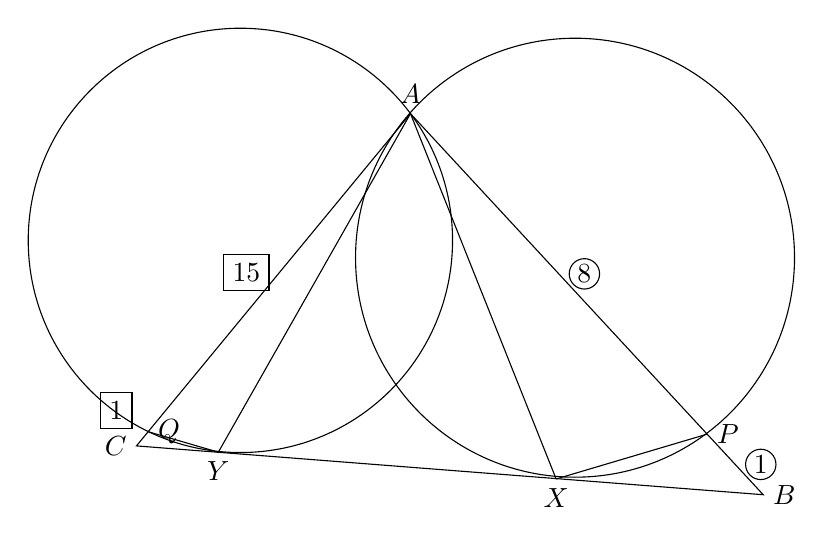
\begin{tikzpicture}
        \coordinate (A) at (-1.48, 4.02);
        \coordinate (B) at (3, -0.82);
        \coordinate (C) at (-4.96, -0.2);
        \coordinate (P) at (2.29, -0.05);
        \coordinate (Q) at (-4.81, -0.02);
        \coordinate (X) at (0.37,-0.62);
        \coordinate (Y) at (-3.92, -0.28);

        \draw (A) -- (B) -- (C) -- cycle;
        \draw (-3.64, 2.41) circle (2.69443871706);
        \draw (0.61, 2.19) circle (2.78747197295);

        \draw (A) -- (Y);
        \draw (A) -- (X);
        \draw (Q) -- (Y);
        \draw (X) -- (P);

        \node[above] at (A) {$A$};
        \node[right] at (B) {$B$};
        \node[left] at (C) {$C$};
        \node[right] at (Q) {$Q$};
        \node[right] at (P) {$P$};
        \node[below] at (Y) {$Y$};
        \node[below] at (X) {$X$};
        \node[right] at ($(A)!0.5!(P)$) {\circled{8}};
        \node[right] at ($(P)!0.5!(B)$) {\circled{1}};
        \node[left] at ($(A)!0.5!(Q)$) {$\boxed{15}$};
        \node[above left] at ($(Q)!0.5!(C)$) {$\boxed{1}$};
    \end{tikzpicture}
\end{center}
    First and foremost, it is evident that $\triangle{BPX}\sim\triangle{BXA}$ and $\triangle{CQY}\sim\triangle{CYA}$. Thereby, the diagram could utilize different variables.
\begin{center}
    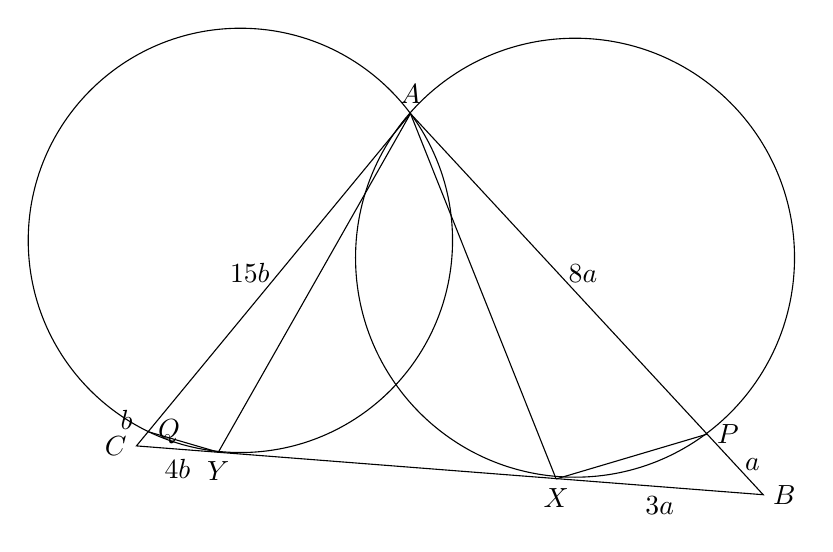
\begin{tikzpicture}
        \coordinate (A) at (-1.48, 4.02);
        \coordinate (B) at (3, -0.82);
        \coordinate (C) at (-4.96, -0.2);
        \coordinate (P) at (2.29, -0.05);
        \coordinate (Q) at (-4.81, -0.02);
        \coordinate (X) at (0.37,-0.62);
        \coordinate (Y) at (-3.92, -0.28);

        \draw (A) -- (B) -- (C) -- cycle;
        \draw (-3.64, 2.41) circle (2.69443871706);
        \draw (0.61, 2.19) circle (2.78747197295);

        \draw (A) -- (Y);
        \draw (A) -- (X);
        \draw (Q) -- (Y);
        \draw (X) -- (P);

        \node[above] at (A) {$A$};
        \node[right] at (B) {$B$};
        \node[left] at (C) {$C$};
        \node[right] at (Q) {$Q$};
        \node[right] at (P) {$P$};
        \node[below] at (Y) {$Y$};
        \node[below] at (X) {$X$};
        \node[right] at ($(A)!0.5!(P)$) {$8a$};
        \node[right] at ($(P)!0.5!(B)$) {$a$};
        \node[left] at ($(A)!0.5!(Q)$) {$15b$};
        \node[above left] at ($(Q)!0.5!(C)$) {$b$};
        \node[below] at ($(C)!0.5!(Y)$) {$4b$};
        \node[below] at ($(X)!0.5!(B)$) {$3a$};
    \end{tikzpicture}
\end{center}
Because the Law of Cosines utilize ratios, if the ratio between $a$ and $b$ are found, $\cos\angle{BAC}$ could also be computed.
\\\\
$AC=CX$ and $AB=BY$ is true. Therefore, $YX=12b=6a$.
\[
\cos\angle{BAC}=\frac{8^2+9^2-11^2}{2\cdot8\cdot9}=\boxed{\frac{1}{6}}
\]
\end{solution}

\end{document}
